\chapter{Nascer, crescer, morrer}\label{ch:g2:born-grow-die}

Na primavera, a cerejeira do portão fica coberta de \omterm{def:g1:plants-around-us:parts}{flores}; embaixo
dela, uma gata amamenta os filhotinhos recém-nascidos; e o vovô
mostra uma foto de quando ele tinha a sua idade --- pequeno, banguela
e já apaixonado por cereja. Todo \omterm{def:g1:living-or-not:living}{ser vivo} percorre a mesma estrada:
ele começa, cresce e um dia acaba. Essa estrada se chama \omterm{def:g2:born-grow-die:cycle}{ciclo de
vida}.

\section{As etapas de uma vida}

\begin{definition}[Ciclo de vida]\label{def:g2:born-grow-die:cycle}
O \emph{ciclo de vida}\index{ciclo de vida} de um \omterm{def:g1:living-or-not:living}{ser vivo} é a
fileira de \emph{etapas}\index{etapa} pelas quais a vida dele passa:
\begin{enumerate}
  \item ele \emph{nasce}\index{nascimento} --- o começo;
  \item ele é \emph{jovem}\index{jovem} --- cresce e muda depressa;
  \item ele é \emph{adulto}\index{adulto} --- totalmente crescido; os
        adultos podem ter filhotes próprios;
  \item ele fica \emph{velho}\index{velhice} e, no fim, ele
        \emph{morre}\index{morte}.
\end{enumerate}
\end{definition}

\begin{example}[Três vidas, a mesma estrada]\label{ex:g2:born-grow-die:three}
Um gatinho nasce, brinca e vira um gato, que talvez tenha gatinhos
também, e fica velho. Um caroço de cereja brota, a árvore jovem
cresce durante anos, a árvore adulta dá \omterm{def:g1:plants-around-us:parts}{flores} e cerejas e, depois de
muitas dezenas de anos, morre. E você: bebê, criança e um dia \omterm{def:g2:born-grow-die:cycle}{adulto}.
Gatinho, cerejeira, criança --- as mesmas quatro \omterm{def:g2:born-grow-die:cycle}{etapas}.
\end{example}

\begin{omfigure}
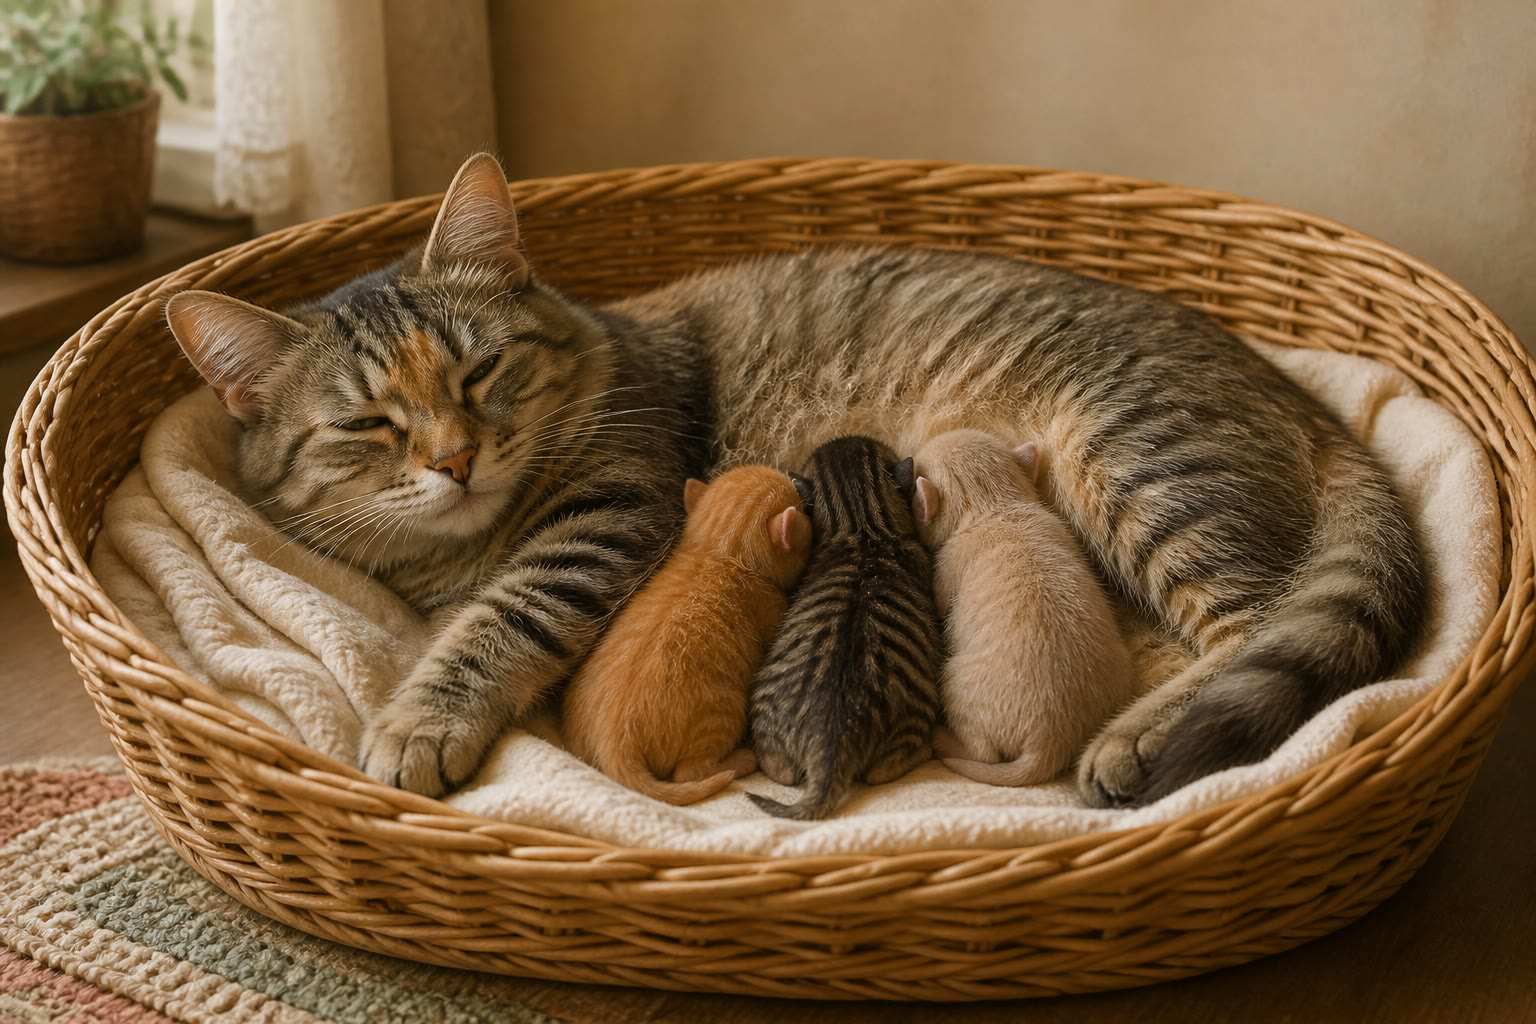
\includegraphics[width=0.62\linewidth]{images/book1/ai/g2-cycle-kittens.jpg}

{\small O começo de três \omterm{def:g2:born-grow-die:cycle}{ciclos de vida} ao mesmo tempo: gatinhos
recém-nascidos mamando na mãe.}
\end{omfigure}

\begin{omfigure}
\begin{tikzpicture}[scale=0.92]
  \foreach \x/\txt in {0/{nascimento},3.1/{jovem},6.2/{adulto},9.3/{velhice}} {
    \draw[thick, omDef, fill=omDef!7, rounded corners=5pt]
      (\x,0) rectangle ({\x+2.4},1.2);
    \node[font=\small\bfseries, text height=1.6ex, text depth=0.4ex]
      at ({\x+1.2},0.6) {\txt};
  }
  \draw[->, thick, omMeth] (2.4,0.6) -- (3.1,0.6);
  \draw[->, thick, omMeth] (5.5,0.6) -- (6.2,0.6);
  \draw[->, thick, omMeth] (8.6,0.6) -- (9.3,0.6);
  % new generation arrow
  \draw[->, thick, omProp] (7.4,1.2) .. controls (7.4,2.3) and (1.2,2.3)
    .. (1.2,1.25);
  \node[font=\small, omProp] at (4.3,2.35) {os adultos têm filhotes: um novo ciclo começa};
\end{tikzpicture}

{\small As \omterm{def:g2:born-grow-die:cycle}{etapas} de uma vida --- e a seta que recomeça a estrada
com a geração seguinte.}
\end{omfigure}

\begin{remark}[Por que se chama ciclo]\label{rem:g2:born-grow-die:wheel}
Cada vida, sozinha, vai do \omterm{def:g2:born-grow-die:cycle}{nascimento} à morte, como uma estrada com
duas pontas. Mas, antes do fim, os \omterm{def:g2:born-grow-die:cycle}{adultos} têm filhotes, e esses
filhotes recomeçam a estrada. Vista ao longo de muitas gerações, a
vida gira como uma roda --- e é por isso que dizemos \emph{ciclo} de
vida.
\end{remark}

\section{Crescer e mudar}

\begin{proposition}[Crescer é mais do que ficar maior]\label{prop:g2:born-grow-die:change}
Enquanto cresce, um \omterm{def:g1:living-or-not:living}{ser vivo} jovem também \emph{muda}: um bebê ganha
dentes, perde esses dentes e ganha outros mais fortes; a penugem
amarela do pintinho vira \omterm{def:g1:animals-around-us:covering}{pena} de verdade; o \omterm{def:g1:plants-around-us:parts}{caule} verde e macio de
uma árvore jovem vira madeira dura. Crescer é ficar maior \emph{e}
ficar diferente.
\end{proposition}
\admitted

\begin{example}[O teste da fotografia]\label{ex:g2:born-grow-die:photo}
Nas fotos antigas do vovô dá para acompanhar uma pessoa em todas as
\omterm{def:g2:born-grow-die:cycle}{etapas}: bebê, criança de escola, rapaz, pai, avô. A mesma pessoa,
com o corpo mudando. As fotografias são pequenas máquinas do tempo
para observar um \omterm{def:g2:born-grow-die:cycle}{ciclo de vida}.
\end{example}

\begin{method}[Pôr as etapas da vida em ordem]\label{met:g2:born-grow-die:order}
Diante de figuras embaralhadas da vida de um \omterm{def:g1:living-or-not:living}{ser vivo}:
\begin{enumerate}
  \item ache a figura do \omterm{def:g2:born-grow-die:cycle}{nascimento} --- ovo, semente ou recém-nascido;
  \item ache o \omterm{def:g2:born-grow-die:cycle}{adulto} --- totalmente crescido, capaz de ter filhotes;
  \item ponha os jovens no meio, do menor para o maior;
  \item confira a sua fileira: cada figura leva à seguinte?
\end{enumerate}
\end{method}

\section{Toda vida acaba --- e a vida continua}

\begin{proposition}[Duração da vida]\label{prop:g2:born-grow-die:lifespan}
\omterm{def:g1:living-or-not:living}{Seres vivos} diferentes vivem por tempos diferentes --- é a
\emph{duração da vida}\index{duração da vida}. Uma borboleta pode
viver algumas semanas; um gato e um cachorro, de dez a vinte anos;
uma pessoa, muitas vezes mais de oitenta anos; algumas árvores,
centenas de anos. Longa ou curta, toda vida tem um fim.
\end{proposition}
\admitted

\begin{example}[A macieira velha]\label{ex:g2:born-grow-die:oldtree}
A macieira velha e torta do fundo do quintal dá menos maçãs a cada
ano --- ela está na \omterm{def:g2:born-grow-die:cycle}{velhice}. Mas as maçãs dela têm sementes, e uma
semente plantada já é uma macieira jovem começando a estrada. Quando
a árvore velha morrer, as macieiras não vão acabar: os filhotes dela
continuam.
\end{example}

\begin{remark}[Falar sobre a morte]\label{rem:g2:born-grow-die:death}
Morrer faz parte de todo \omterm{def:g2:born-grow-die:cycle}{ciclo de vida}, e tudo bem ficar triste com
isso --- as pessoas ficam, principalmente com os bichinhos de
estimação e com as pessoas que amam. A \omterm{def:g1:living-or-not:living}{biologia} traz um consolo:
como os \omterm{def:g2:born-grow-die:cycle}{adultos} têm filhotes antes de morrer, a própria vida
continua, ciclo após ciclo.
\end{remark}

\section{Exercícios}

\begin{exercise}[$\star$]\label{exo:g2:born-grow-die:1}
Diga as quatro \omterm{def:g2:born-grow-die:cycle}{etapas} de um \omterm{def:g2:born-grow-die:cycle}{ciclo de vida}, em ordem.
\end{exercise}

\begin{exercise}[$\star$]\label{exo:g2:born-grow-die:2}
Em qual \omterm{def:g2:born-grow-die:cycle}{etapa} um \omterm{def:g1:living-or-not:living}{ser vivo} pode ter filhotes próprios?
\end{exercise}

\begin{exercise}[$\star$]\label{exo:g2:born-grow-die:3}
Ponha em ordem, do mais velho para o mais novo: uma criança de
escola, um bebê, uma avó, uma mãe.
\end{exercise}

\begin{exercise}[$\star$]\label{exo:g2:born-grow-die:4}
Dê o \omterm{def:g2:born-grow-die:cycle}{ciclo de vida} da cerejeira do \cref{ex:g2:born-grow-die:three},
\omterm{def:g2:born-grow-die:cycle}{etapa} por \omterm{def:g2:born-grow-die:cycle}{etapa}.
\end{exercise}

\begin{exercise}[$\star$]\label{exo:g2:born-grow-die:5}
Dê dois exemplos da \cref{prop:g2:born-grow-die:change} de um \omterm{def:g1:living-or-not:living}{ser
vivo} jovem que \emph{muda} enquanto cresce, e não só fica maior.
\end{exercise}

\begin{exercise}[$\star$]\label{exo:g2:born-grow-die:6}
Quem costuma viver mais tempo: uma borboleta, um gato ou um
carvalho? Ponha os três em ordem de \omterm{prop:g2:born-grow-die:lifespan}{duração da vida}.
\end{exercise}

\begin{exercise}[$\star$]\label{exo:g2:born-grow-die:7}
Por que se usa a palavra \emph{ciclo}, se cada vida sozinha vai do
\omterm{def:g2:born-grow-die:cycle}{nascimento} à morte como uma estrada? Use a seta roxa da figura.
\end{exercise}

\begin{exercise}[$\star$]\label{exo:g2:born-grow-die:8}
Faça a experiência: peça à sua família fotos de um \omterm{def:g2:born-grow-die:cycle}{adulto} em idades
diferentes e ponha as fotos em ordem de \omterm{def:g2:born-grow-die:cycle}{ciclo de vida} com o
\cref{met:g2:born-grow-die:order}. Que \omterm{def:g2:born-grow-die:cycle}{etapas} as fotos mostram? Qual
\omterm{def:g2:born-grow-die:cycle}{etapa} ainda está por vir?
\end{exercise}

\begin{exercise}[$\star\star$]\label{exo:g2:born-grow-die:9}
A macieira velha do \cref{ex:g2:born-grow-die:oldtree} vai morrer um
dia, e mesmo assim o quintal não precisa ficar sem macieiras.
Explique por quê, usando a palavra \emph{geração} ou a seta roxa da
figura.
\end{exercise}

\begin{exercise}[$\star\star$]\label{exo:g2:born-grow-die:10}
Uma pedrinha nunca morre. Será que é porque ela é muito forte? Use a
ideia de vivo e não vivo do \cref{ch:g1:living-or-not} para explicar.
\end{exercise}
